\documentclass[tikz, preview]{standalone}

\usepackage{amsfonts, amsthm, amssymb, amsmath, stmaryrd, etoolbox}
\usepackage{tikz}
\usetikzlibrary{matrix,arrows}

\begin{document}
\[
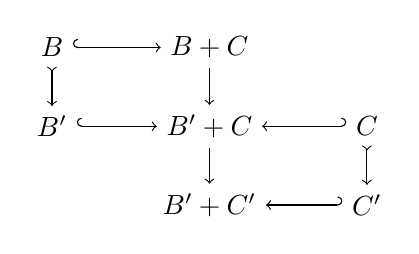
\begin{tikzpicture}
\node (B) at (-2,1) {$B$};
\node (B') at (-2,0) {$B'$};
\node (BC) at (0,1) {$B+C$};
\node (B'C) at (0,0) {$B'+C$};
\node (B'C') at (0,-1) {$B'+C'$};
\node (C) at (2,0) {$C$};
\node (C') at (2,-1) {$C'$};
%
\draw [right hook->] (B) edge (BC);
\draw [>->] (B) edge (B');
\draw [right hook->] (B') edge (B'C);
\draw [->] (BC) edge (B'C);
\draw [->] (B'C) edge (B'C');
\draw [left hook->] (C) edge (B'C);
\draw [>->] (C) edge (C');
\draw [left hook->] (C') edge (B'C');
\end{tikzpicture}
\]
\end{document}
